\chapter{Teknologi}
I dette afsnit undersøges Ultralyds Robotarmen ud fra et teknologisk perspektiv. Den teknologiske løsning Ultralyds Robotarm består af:
\begin{itemize}
\item  Delta robot incl. software til styring af denne
\item Stativ til robotten
\item Joystick
\item Computer
\item Holder til ultralydsprobe
\item Kameraer
\end{itemize}
Denne løsning skal kobles til det allerede eksisterende udstyr. Derfor er produktet en add-on løsning. Hvilket betyder at produktet skal købes udover det almindelige udstyr. Se bilag --- (ØKONOMI)
\begin{figure}[h!]\centering
	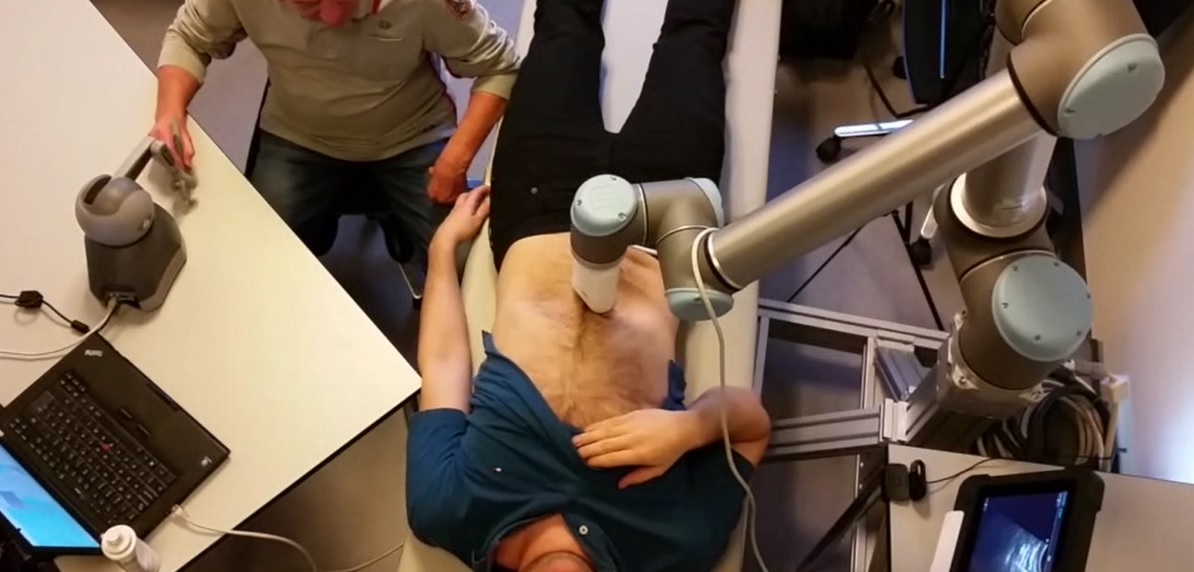
\includegraphics[width = 1.0\textwidth]{Figurer/ergonomiskLosning.jpg}
	\caption{Eksempel på opstilling af Ultralyds Robotarm.}
	\label{ergonomiskLosning}
\end{figure}

\begin{figure}[h!]\centering
	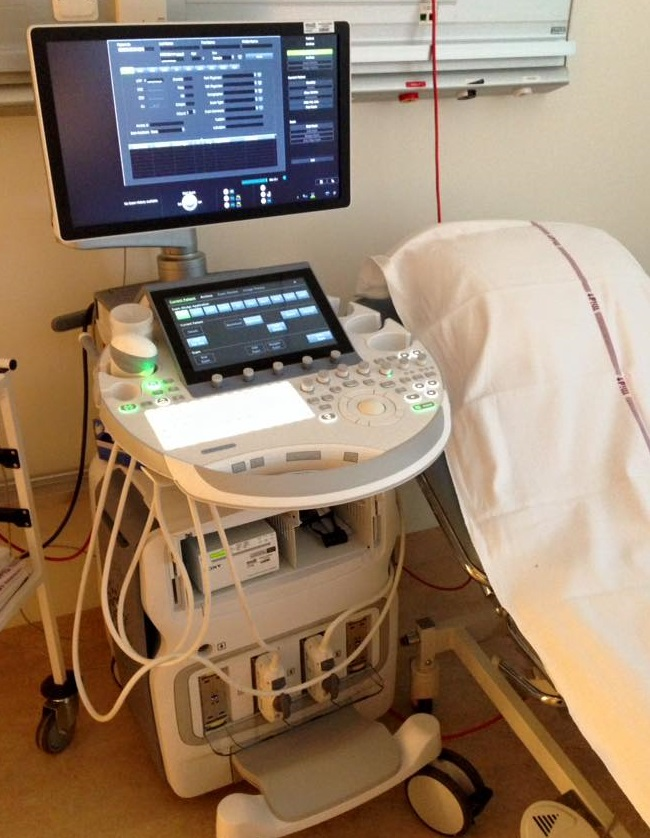
\includegraphics[width = 0.5\textwidth]{Figurer/udstyrHorsens.jpg}
	\caption{Eksempel på ultralydsudstyr fra Horsens.}
	\label{udstyrHorsens}
\end{figure}


\section{Anvendelsesområde}
Produktet skal anvendes til ultralydsscanninger af gravide borgere.
På robotarmen findes en holder til ultralydsproben. 
Robotarmen skal holde ultralydsproben over den gravide, mens den styres af sonografen via et joystick. Derved behøver sonografen ikke selv at styre proben og akavede arbejdsstillinger undgås. 
Gravide kvinder
BMI-problem
\section{Effektivitet}
BMI-problem
Ændrer ikke på produktet - altså samme scanning (der bruges de samme prober)
Tryk - hvordan registreres dette.
\section{Risikovurdering}
pålidelighed
før vs. nu
forbedring af arbejdsstillinger